% Created 2022-07-26 Tue 15:32
% Intended LaTeX compiler: xelatex
\documentclass[10pt,a4paper,nobib]{tufte-handout}
\usepackage{fontspec}
\usepackage{graphicx}
\usepackage{longtable}
\usepackage{wrapfig}
\usepackage{rotating}
\usepackage[normalem]{ulem}
\usepackage{amsmath}
\usepackage{amssymb}
\usepackage{capt-of}
\usepackage{hyperref}
\usepackage{booktabs}
\usepackage{microtype}
\usepackage{newunicodechar}
\usepackage[notions,operators,sets,keys,ff,adversary,primitives,complexity,asymptotics,lambda,landau,advantage]{cryptocode}
\usepackage[capitalize]{cleveref}
\usepackage[british]{babel}
\usepackage{xspace}
\usepackage{units}
\usepackage{nicefrac}
\usepackage{gensymb}
\usepackage{amsthm}
\usepackage{amsmath}
\usepackage{amssymb}
\usepackage{xcolor}
\usepackage{listings}
\usepackage[color=cyan!0!magenta!4!yellow!16]{todonotes}
\makeatletter
\patchcmd{\@verbatim}
  {\verbatim@font}
  {\verbatim@font\scriptsize}
  {}{}
\makeatother

\newunicodechar{ }{~}
\newtheorem{lemma}{Lemma}
\newtheorem{theorem}{Theorem}
\newtheorem{definition}{Definition}
\newtheorem{remark}{Remark}
\newtheorem{corollary}{Corollary}
\newtheorem{proposition}{Proposition}

\DeclareMathOperator{\Vol}{Vol}
\DeclareMathOperator{\GH}{GH}
\renewcommand{\vec}[1]{\ensuremath{\mathbf{#1}}\xspace}
\renewcommand{\norm}[1]{\left\lVert#1\right\rVert}
\providecommand{\mat}[1]{\ensuremath{\vec{#1}}\xspace}
\providecommand{\ring}[0]{\ensuremath{\mathcal{R}}\xspace}


\newcommand{\malb}[2][inline]{\todo[#1]{\textbf{malb:} #2}\xspace}

\lstdefinelanguage{Sage}[]{Python}{
   morekeywords={True,False,sage,cdef,cpdef,ctypedef,self},
   sensitive=true
}

\lstdefinelanguage{diff}{
  morecomment=[f][\color{black}\textbf]{+\ },
  morecomment=[f][\color{darkgray}]{-\ },
}

\lstset{showtabs=False,
        showspaces=False,
        showstringspaces=False,
        commentstyle={\color{gray}},
        keywordstyle={\color{black}\textbf},
        stringstyle={\color{darkgray}},
        frame=single,
        basicstyle=\tt\scriptsize\relax,
        inputencoding=utf8,
        literate={…}{{\ldots}}1,
        belowskip=0.0em,}


\IfFontExistsTF{Cousine}{
\setmonofont[BoldFont={Cousine Bold},
             ItalicFont={Cousine Italic},
             BoldItalicFont={Cousine Bold Italic},
             Scale=0.90]{Cousine}
}{}

\IfFontExistsTF{TeX Gyre Pagella}{
\setmainfont{TeX Gyre Pagella}
}{}

\linespread{1.04}

\IfFileExists{unicodesymbols.sty}{
\RequirePackage{unicodesymbols} % after metropolis which loads fontspec
}{}

% \usepackage{unicode-math}

\usepackage{ifxetex}
\ifxetex
 \renewcommand{\textls}[2][5]{%
 \begingroup\addfontfeatures{LetterSpace=#1}#2\endgroup
}
\renewcommand{\allcapsspacing}[1]{\textls[15]{#1}}
\renewcommand{\smallcapsspacing}[1]{\textls[10]{#1}}
\renewcommand{\allcaps}[1]{\textls[15]{\MakeTextUppercase{#1}}}
\renewcommand{\smallcaps}[1]{\smallcapsspacing{\scshape\MakeTextLowercase{#1}}}
\renewcommand{\textsc}[1]{\smallcapsspacing{\textsmallcaps{#1}}}
\usepackage{fontspec}
\fi
\lstset{showstringspaces=false,
aboveskip=0.75em,
basicstyle=\footnotesize\ttfamily,
keywordstyle=\bfseries\color{gray!40!black},
commentstyle=\itshape\color{gray!140!black},
identifierstyle=\color{gray!40!black},
stringstyle=\color{gray},
backgroundcolor=\color{gray!190!black},
frame=none,
}
\usepackage[backend=bibtex,
style=alphabetic,
maxnames=8,
citestyle=alphabetic]{biblatex}
\bibliography{local,abbrev3,crypto_crossref}
\addtolength{\topmargin}{-6.0pt}
\author{Martin R. Albrecht}
\date{27 July 2022}
\title{Lattice Reduction \& Attacks\\\medskip
\large Lab}
\hypersetup{
pdfauthor={Martin R. Albrecht},
pdftitle={Lattice Reduction \& Attacks},
pdfkeywords={},
pdfsubject={},
pdfcreator={Emacs 28.1.90 (Org mode 9.5.4)},
pdflang={British},
colorlinks,
citecolor=gray,
filecolor=gray,
linkcolor=gray,
urlcolor=gray
}
\begin{document}

\maketitle
In this lab, we will make intensive use of FPLLL and FPyLLL.

\begin{description}
\item[{FPLLL}] is a C++11 library for operating on lattices using floating point arithmetic. It implements Gram-Schmidt orthogonalisation, LLL, BKZ, BKZ 2.0 \footfullcite{AC:CheNgu11}, Slide reduction \footfullcite{STOC:GamNgu08} and Self-Dual BKZ \footfullcite{EPRINT:MicWal15}.

\item[{FPyLLL}] is a Python wrapper and extension of FPLLL, making its data structures and algorithms available in Python and \href{https://sagemath.org}{SageMath}. It also (re-)implements some algorithms in Python to make their internals easily accessible, a feature we will make use of.

\item[{G6K}] is C++ library \& Python wrapper that implements lattice sieving. This tutorial \emph{should} use G6K but it does not come by default with SageMath. Thus, to avoid spending all our time installing it, this lab uses only FPLLL/FPyLLL. Feel encouraged to try these exercised with G6K later, which builds on FPyLLL.
\end{description}

\section{Introduction}
\label{sec:org94c7593}
In this lab, we ask you to experiment with LLL and BKZ as implemented in FPyLLL. We start with a little tutorial on how to use this library.  To start, we first import the \texttt{fpylll} API into Sage’s main namespace:
\lstset{language=Python,label= ,caption= ,captionpos=b,numbers=none}
\begin{lstlisting}
from fpylll import *
\end{lstlisting}

\subsection{Integer Matrices}
\label{sec:org4d93d76}

To experiment, we generate a \(q\)-ary lattice of dimension 100 and determinant \(q^{50}\) where \(q\) is a 30-bit prime. Before we sample our basis, we set the random seed to ensure we can reproduce our experiments later.

\lstset{language=Python,label= ,caption= ,captionpos=b,numbers=none}
\begin{lstlisting}
set_random_seed(1337)
A = IntegerMatrix.random(100, "qary", k=50, bits=30)
\end{lstlisting}

\begin{remark}
Objects and functions in Python/Sage can be interrogated to learn more about them such as what parameters they accept (for functions) or (often) their \href{https://doc.sagemath.org/html/en/tutorial/tour\_help.html}{documentation}.
\end{remark}

\subsection{Gram–Schmidt Orthogonalisation}
\label{sec:org206f313}

To run LLL we have two choices. We can either run the high-level \texttt{LLL.reduction()} function or we can create the appropriate hierarchy of objects “by hand”. That is, algorithms are represented by objects with which we can interact. As this exercise is about dealing with those internal objects, we are going to pursue this strategy. We, hence, first create a \texttt{MatGSO} object, which takes care of computing the Gram-Schmidt orthogonalisation. A \texttt{MatGSO} object stores the following information:
\begin{itemize}
\item An integral basis \(\mat{B}\),
\item the Gram--Schmidt coefficients \(μ_{i,j} = ⟨\vec{b}_i, \vec{b}^*_j⟩ / \|\vec{b}^*_j\|^2\) for \(i>j\),
\item the coefficients \(r_{i,j} = ⟨\vec{b}_i, \vec{b}^*_j⟩ = μ_{i,j} ⋅ r_{j,j}\) for \(i\geq j\)
\end{itemize}
It holds that: \(\mat{B} = \mat{R} × \mat{Q} = (\mat{μ} × \mat{D}) × (\mat{D}^{-1} × \mat{B}^*)\) where \(\mat{Q}\) is orthonormal, \(\mat{R}\) is lower triangular and \(\mat{B}^*\) is the Gram-Schmidt orthogonalisation.

We choose the floating point type (≈ bits of precision) used to represent the Gram-Schmidt coefficients as native \texttt{double}, which is fastest and fine up to dimension 170 or so. If you choose \texttt{mpfr} for arbitrary precision, you must call \texttt{FPLLL.set\_precision(prec)} before constructing your object \texttt{M}, i.e. precision is global!

\lstset{language=Python,label= ,caption= ,captionpos=b,numbers=none}
\begin{lstlisting}
M = GSO.Mat(A, float_type="d")
\end{lstlisting}

When we said “internal”, we meant it. Note that \texttt{M} is lazy, i.e. the Gram--Schmidt orthogonalisation is only computed/updated when needed. For example, as of now, none of the coefficients are meaningful:
\lstset{language=Python,label= ,caption= ,captionpos=b,numbers=none}
\begin{lstlisting}
M.get_r(0,0)
\end{lstlisting}

\begin{verbatim}
0.0
\end{verbatim}


To get meaningful results, we need to trigger the appropriate computation. To compute the complete GSO, run:

\lstset{language=Python,label= ,caption= ,captionpos=b,numbers=none}
\begin{lstlisting}
_ = M.update_gso()
\end{lstlisting}

This is better:
\lstset{language=Python,label= ,caption= ,captionpos=b,numbers=none}
\begin{lstlisting}
M.get_r(0,0)/A[0].norm()^2  
\end{lstlisting}

\begin{verbatim}
1.0
\end{verbatim}


You can call \texttt{update\_gso} at construction time with:
\lstset{language=Python,label= ,caption= ,captionpos=b,numbers=none}
\begin{lstlisting}
M = GSO.Mat(A, float_type="d", update=True)
\end{lstlisting}

\begin{remark}
FP(y)LLL also supports GSO objects for Gram matrices, i.e. in lieu of a basis.
\end{remark}

\subsection{LLL}
\label{sec:org64152f7}

We can now create an LLL object which operates on GSO objects. All operations performed on GSO objects, e.g. \texttt{M}, are automatically also applied to the underlying integer matrix, e.g. \texttt{A}.
\lstset{language=Python,label= ,caption= ,captionpos=b,numbers=none}
\begin{lstlisting}
L = LLL.Reduction(M, delta=0.99, eta=0.501, flags=LLL.VERBOSE)
\end{lstlisting}

Now that we have an LLL object, we can call it, i.e. run the algorithm. Note that you can specify a range of rows on which to perform LLL.
\lstset{language=Python,label= ,caption= ,captionpos=b,numbers=none}
\begin{lstlisting}
L(0, 0, 10)
\end{lstlisting}

\begin{verbatim}
Entering LLL
delta = 0.99
eta = 0.501
precision = 53
exact_dot_product = 0
row_expo = 0
early_red = 0
siegel_cond = 0
long_in_babai = 0
Discovering vector 2/10 cputime=0
Discovering vector 3/10 cputime=0
Discovering vector 4/10 cputime=0
Discovering vector 5/10 cputime=0
Discovering vector 6/10 cputime=0
Discovering vector 7/10 cputime=0
Discovering vector 8/10 cputime=0
Discovering vector 9/10 cputime=0
Discovering vector 10/10 cputime=0
End of LLL: success
\end{verbatim}

That’s maybe a bit verbose, let’s continue to the end without all that feedback:

\lstset{language=Python,label= ,caption= ,captionpos=b,numbers=none}
\begin{lstlisting}
L = LLL.Reduction(M, delta=0.99, eta=0.501)  
L()
\end{lstlisting}

If our LLL implementation is any good, then \(\|μ_{i,j}\| ≤ η\) should hold for all \(i>j\). Let’s check:
\lstset{language=Python,label= ,caption= ,captionpos=b,numbers=none}
\begin{lstlisting}
all([abs(M.get_mu(i,j)) <= 0.501 for i in range(M.d) for j in range(i)])
\end{lstlisting}

\begin{verbatim}
True
\end{verbatim}


We also want to check if we made progress on \texttt{A}:
\lstset{language=Python,label= ,caption= ,captionpos=b,numbers=none}
\begin{lstlisting}
A[0].norm()^2
\end{lstlisting}

\begin{verbatim}
57755566272.00001
\end{verbatim}

\subsection{BKZ}
\label{sec:org8167ef7}

Calling BKZ works similarly: there is a high-level function \texttt{BKZ.reduction()} and a BKZ object \texttt{BKZ.Reduction}. However, in addition there are also several implementations of the BKZ algorithm in 
\begin{verbatim}
fpylll.algorithms
\end{verbatim}
These are re-implementations of BKZ-syle algorithms in Python which makes them rather hackable, i.e. we can modify different parts of the algorithms relatively easily. To use those, we first have to import them. We opt for BKZ 2.0:\footnote{See \href{https://github.com/fplll/fpylll/blob/master/src/fpylll/algorithms/simple\_bkz.py}{here} for a simple implementation of BKZ.}

\lstset{language=Python,label= ,caption= ,captionpos=b,numbers=none}
\begin{lstlisting}
from fpylll.algorithms.bkz2 import BKZReduction as BKZ2
\end{lstlisting}

BKZ 2.0 takes a lot of parameters, such as:
\begin{description}
\item[{\texttt{block\_size}}] the block size
\item[{\texttt{strategies}}] we explain this one below
\item[{\texttt{flags}}] verbosity, early abort, etc.
\item[{\texttt{max\_loops}}] limit the number of tours
\item[{\texttt{auto\_abort}}] heuristic, stop when the average slope of \(\log(\|b_i^*\|)\) does not decrease fast enough
\item[{\texttt{gh\_factor}}] heuristic, if set then the enumeration bound will be set to this factor times the Gaussian Heuristic.
\end{description}
It gets old fast passing these around one-by-one. Thus, FPLLL and FPyLLL introduce an object \texttt{BKZ.Param} to collect such parameters:

\lstset{language=Python,label= ,caption= ,captionpos=b,numbers=none}
\begin{lstlisting}
flags = BKZ.AUTO_ABORT|BKZ.MAX_LOOPS|BKZ.GH_BND 
params = BKZ.Param(60, strategies=BKZ.DEFAULT_STRATEGY,
                   max_loops=4,
                   flags=flags)
\end{lstlisting}

The parameter \texttt{strategies} takes a list of “reduction strategies” or a filename for a JSON file containing such strategies. For each block size these strategies determine what pruning coefficients are used and what kind of recursive preprocessing is applied before enumeration. The strategies in \texttt{BKZ.DEFAULT\_STRATEGY} were computed using fplll’s \href{https://github.com/fplll/strategizer}{\texttt{strategizer}}.

\lstset{language=Python,label= ,caption= ,captionpos=b,numbers=none}
\begin{lstlisting}
strategies = load_strategies_json(BKZ.DEFAULT_STRATEGY)
print(strategies[60])
\end{lstlisting}

\begin{verbatim}
Strategy< 60, (40), 0.30-0.53, {}>
\end{verbatim}


That last line means that for block size 60 we are preprocessing with block size 40 and our pruning parameters are such that enumeration succeeds with probability between 29\% and 50\% depending on the target enumeration radius. Still, constructing such parameter objects gets old, too, we can simply call:
\lstset{language=Python,label= ,caption= ,captionpos=b,numbers=none}
\begin{lstlisting}
params = BKZ.EasyParam(60, max_loops=4)
\end{lstlisting}

Finally, let’s call BKZ-60 on our example lattice:
\lstset{language=Python,label= ,caption= ,captionpos=b,numbers=none}
\begin{lstlisting}
bkz = BKZ2(A) # or
bkz = BKZ2(GSO.Mat(A)) # or 
bkz = BKZ2(LLL.Reduction(GSO.Mat(A)))

_ = bkz(params)
\end{lstlisting}

\section{Lattice Reduction}
\label{sec:org0bdc19b}

In this exercise, we ask you to verify various predictions made about lattice reduction using the implementations available in FPyLLL.

\subsection{root-Hermite factors}
\label{sec:org89f91b1}

Recall that lattice reduction returns vectors such that
\[
\|\vec{v}\| = δ^{d-1} ⋅ \Vol(\Lambda)^{1/d}
\]
where \(\delta\) is the root-Hermite factor which depends on the algorithm. For LLL it  is \(δ_0≈1.0219\) and for BKZ-\(k\) it is \[δ_0 ≈ \left( \frac{k}{2 π e} (π k)^{\frac{1}{k}}  \right)^{\frac{1}{2(k-1)}}.\] Experimentally measure root-Hermite factors for various bases and algorithms.

\subsection{GS norms \& Geometric series assumption}
\label{sec:org53b0511}

Schnorr’s geometric series assumption (GSA) states that the norms of the Gram-Schmidt vectors after lattice reduction satisfy \[\|\vec{b}_i^*\| = {α_\beta}^{(d-1-2i)/2} ⋅ \Vol(\Lambda)^{1/d} \textnormal{ for some } 0 < α_{\beta} < 1\]
and \(\alpha_\beta = {\mathrm{GH}(\beta)}^{1/(\beta-1)}\).

Check how well this assumption holds for various block sizes of BKZ. That is, running several tours of BKZ 2.0, plot the logs of Gram-Schmidt norms agains the GSA after each tour. You have several options to get to those norms:
\begin{itemize}
\item Check out the \texttt{dump\_gso\_filename} option for \texttt{BKZ.Param}.
\item Set up BKZ parameters to run one tour only an measure between BKZ calls.
\item Inherit from \texttt{fpylll.algorithms.bkz2.BKZReduction} and add the functionality to plot after each tour.
\end{itemize}
To plot you can simply call \texttt{line()} to plot, e.g. 
\lstset{language=Python,label= ,caption= ,captionpos=b,numbers=none}
\begin{lstlisting}
kwds = {"color": "lightgrey", "dpi":150r, "thickness":2}
line(zip(range(10),prime_range(30)), **kwds)
\end{lstlisting}

\begin{center}
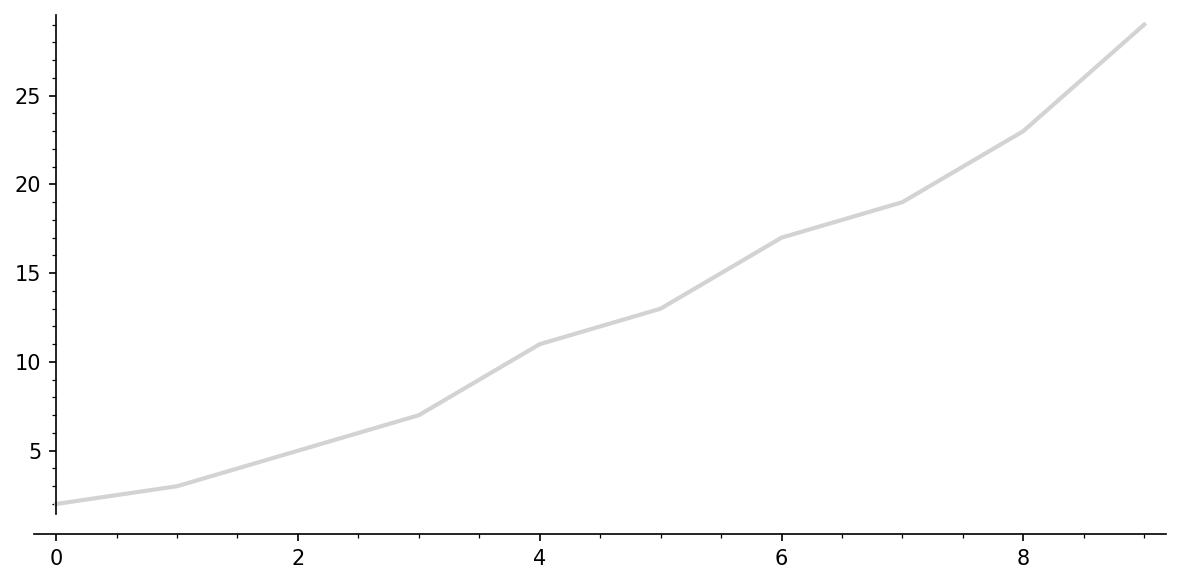
\includegraphics[width=.9\linewidth]{lab-plot-line-sage.png}
\end{center}

\section{Primal Attack}
\label{sec:org158e6b7}

For varying parameters \((n,q,\chi_{e})\) determine the BKZ block size required to break LWE instances corresponding to these parameters and compare your predict with experimental evidence. You may use the following lattice basis generator to run those experiments.

\lstset{language=Python,label= ,caption= ,captionpos=b,numbers=none}
\begin{lstlisting}
def lwe_instancef(n=20, q=7681, Xe=2, Xs=None, m=None):
    m = n if m is None else m
    Xs = Xe if Xs is None else Xs
    s = random_vector(ZZ, n, x=-Xs, y=Xs+1)
    e = random_vector(ZZ, m, x=-Xe, y=Xe+1)
    A = random_matrix(GF(q), m, n)
    b = A*s + e
    B = block_matrix(
        [
            [q*identity_matrix(ZZ, m), 0, 0],
            [A.T.lift(),identity_matrix(ZZ, n),0],
            [matrix(ZZ,1,m,b).lift(), 0, Xe],
        ])
    return B

B = lwe_instancef()
\end{lstlisting}


\appendix
\clearpage

\section{Example Solutions}
\label{sec:org98f96ec}
\subsection{root-Hermite factors}
\label{sec:orgd7cdc74}

\lstset{language=Python,label= ,caption= ,captionpos=b,numbers=none}
\begin{lstlisting}
# -*- coding: utf-8 -*-
from fpylll import *

deltaf = lambda b: (b/(2*pi*e) * (pi*b)^(1/b))^(1/(2*b-1))
fmt = "n: %3d, bits: %2d, β: %2d, δ_0: %.4f, " \
    + "pred: 2^%5.2f, real: 2^%5.2f"

N = (50, 70, 90, 110, 130)
BETAS = (2, 20, 50, 60)
q = 7681

ntrials = 8
for n in N:
    for beta in BETAS:
        if beta > n:
            continue
        delta = 1.0219 if beta == 2 else deltaf(beta)
        n_pred = float(delta^(n-1) * q^(1/2))
        n_real = []
        for i in range(ntrials):
            A = IntegerMatrix.random(n, "qary", k=n/2, q=q)
            if beta == 2:
                LLL.reduction(A)
            else:
                BKZ.reduction(A, BKZ.EasyParam(block_size=beta))
            n_real.append(A[0].norm())
        n_real = sum(n_real)/ntrials
        print(fmt%(n, bits, beta, delta,
                   log(n_pred,2), log(n_real,2)))
\end{lstlisting}

\begin{verbatim}
n:  50, bits: 20, β:  2, δ_0: 1.0219, pred: 2^ 7.98, real: 2^ 7.73
n:  50, bits: 20, β: 20, δ_0: 1.0094, pred: 2^ 7.11, real: 2^ 7.40
n:  50, bits: 20, β: 50, δ_0: 1.0119, pred: 2^ 7.29, real: 2^ 7.31
n:  70, bits: 20, β:  2, δ_0: 1.0219, pred: 2^ 8.61, real: 2^ 8.53
n:  70, bits: 20, β: 20, δ_0: 1.0094, pred: 2^ 7.38, real: 2^ 7.82
n:  70, bits: 20, β: 50, δ_0: 1.0119, pred: 2^ 7.64, real: 2^ 7.56
n:  70, bits: 20, β: 60, δ_0: 1.0114, pred: 2^ 7.58, real: 2^ 7.54
n:  90, bits: 20, β:  2, δ_0: 1.0219, pred: 2^ 9.24, real: 2^ 8.96
n:  90, bits: 20, β: 20, δ_0: 1.0094, pred: 2^ 7.65, real: 2^ 8.27
n:  90, bits: 20, β: 50, δ_0: 1.0119, pred: 2^ 7.98, real: 2^ 7.93
n:  90, bits: 20, β: 60, δ_0: 1.0114, pred: 2^ 7.90, real: 2^ 7.87
n: 110, bits: 20, β:  2, δ_0: 1.0219, pred: 2^ 9.86, real: 2^ 9.62
n: 110, bits: 20, β: 20, δ_0: 1.0094, pred: 2^ 7.92, real: 2^ 8.72
n: 110, bits: 20, β: 50, δ_0: 1.0119, pred: 2^ 8.32, real: 2^ 8.26
n: 110, bits: 20, β: 60, δ_0: 1.0114, pred: 2^ 8.23, real: 2^ 8.19
n: 130, bits: 20, β:  2, δ_0: 1.0219, pred: 2^10.49, real: 2^10.41
n: 130, bits: 20, β: 20, δ_0: 1.0094, pred: 2^ 8.19, real: 2^ 9.10
n: 130, bits: 20, β: 50, δ_0: 1.0119, pred: 2^ 8.66, real: 2^ 8.64
n: 130, bits: 20, β: 60, δ_0: 1.0114, pred: 2^ 8.56, real: 2^ 8.50
\end{verbatim}

\subsection{GS norms \& Geometric series assumption}
\label{sec:orgd4bb373}

\texttt{dump\_gso\_filename}

\lstset{language=Python,label= ,caption= ,captionpos=b,numbers=none}
\begin{lstlisting}
# -*- coding: utf-8 -*-
from fpylll import *

set_random_seed(1)
n, bits = 120, 40
A = IntegerMatrix.random(n, "qary", k=n/2, bits=bits)
beta = 60
tours = 8

fn = "/tmp/logs.txt"
par = BKZ.EasyParam(block_size=beta,
                dump_gso_filename=fn,
                max_loops=tours)

delta = (beta/(2*pi*e) * (pi*beta)^(1/ZZ(beta)))^(1/(2*beta-1))
alpha = delta^(-2*n/(n-1))

norms = [map(log, [(alpha^i * delta^n * 2^(bits/2))^2
                   for i in range(n)])]

BKZ.reduction(A, par)

for i, l in enumerate(open(fn).readlines()):
    if i > tours:
        break
    _norms =  l.split(":")[1] # stop off other information
    _norms = _norms.strip().split(" ") # split string
    _norms = map(float, _norms) # map to floats
    norms.append(_norms)
        
C = ["#4D4D4D", "#5DA5DA", "#FAA43A", "#60BD68", 
           "#F17CB0", "#B2912F", "#B276B2", "#DECF3F", "#F15854"]

g  = line(zip(range(n), norms[0]), legend_label="GSA", color=C[0])
g += line(zip(range(n), norms[1]), legend_label="lll", color=C[1])

for i,_norms in enumerate(norms[2:]):
    g += line(zip(range(n), _norms), 
              legend_label="tour %d"%i, color=C[i+2])
g
\end{lstlisting}

\texttt{bkz.tour}

\lstset{language=Python,label= ,caption= ,captionpos=b,numbers=none}
\begin{lstlisting}
# -*- coding: utf-8 -*-
from fpylll import *
from fpylll.algorithms.bkz2 import BKZReduction as BKZ2

set_random_seed(1)
n, bits = 120, 40
A = IntegerMatrix.random(n, "qary", k=n/2, bits=bits)
beta = 60
tours = 2
par = BKZ.EasyParam(block_size=beta)

delta = (beta/(2*pi*e) * (pi*beta)^(1/ZZ(beta)))^(1/(2*beta-1))
alpha = delta^(-2*n/(n-1))

LLL.reduction(A)

M = GSO.Mat(A)
M.update_gso()


norms  = [map(log, [(alpha^i * delta^n * 2^(bits/2))^2
                    for i in range(n)])]
norms += [[log(M.get_r(i,i)) for i in range(n)]]

bkz = BKZ2(M)

for i in range(tours):
    bkz.tour(par)
    norms += [[log(M.get_r(i,i)) for i in range(n)]]
        
C = ["#4D4D4D", "#5DA5DA", "#FAA43A", "#60BD68", 
           "#F17CB0", "#B2912F", "#B276B2", "#DECF3F", "#F15854"]

g  = line(zip(range(n), norms[0]), legend_label="GSA", color=C[0])
g += line(zip(range(n), norms[1]), legend_label="lll", color=C[1])

for i,_norms in enumerate(norms[2:]):
    g += line(zip(range(n), _norms), 
              legend_label="tour %d"%i, color=C[i+2])
g
\end{lstlisting}
\end{document}